\chapter{Boxicity of CA graphs}\label{ch:cabox}
  In this chapter\footnote{Joint work with Abhijin Adiga and L. Sunil Chandran. An initial version of this work was presented in WADS 2011. 
A complete version is under revision in Discrete Applied Mathematics.}, we consider the problem of approximating the boxicity (resp. cubicity) of circular arc graphs - intersection graphs of arcs of a circle. Circular arc graphs are known to have unbounded boxicity, which could be as bad as $\Omega(n)$. We give a $\left(2+\frac{1}{k}\right)$-factor (resp. $\left(2+\frac{\lceil\log{n}\rceil}{k}\right)$-factor) polynomial time approximation algorithm for computing the boxicity (resp. cubicity) of any circular arc graph, where $k$ is the value of the optimum solution. For normal circular arc (NCA) graphs, with an NCA model given, this can be improved to an additive two approximation algorithm. The time complexity of the algorithms to approximately compute the boxicity (resp. cubicity) is $O(mn+n^2)$ in both these cases, where $n$ is the number of vertices of the graph and 
$m$ is its number of edges. In $O(mn+kn^2)= O(n^3)$ time we get their corresponding box (resp. cube) representations. Our additive two approximation algorithm directly works for any 
proper circular arc graph, since their NCA models can be computed in polynomial time.

This seems to be the first result obtaining a polynomial time algorithm with a sublinear approximation factor for computing boxicity, 
of any well known graph class of unbounded boxicity. 
%\end{quote}
\section{Introduction} \label{sec:intro}
%\paragraph{Boxicity}
Let $G(V$, $E)$ be a graph. Recall that we defined a $d$-dimensional box (resp. cube) representation of $G$ as a 
geometric representation where each vertex is associated with an axis parallel box (resp. axis parallel unit hypercube) in $\mathbb{R}^k$ so that 
two boxes (resp. hypercubes) intersect if and only if the corresponding vertices are adjacent in $G$. 
It is easy to see that projecting this geometric representation to any of the $d$ coordinate axes gives an interval (resp. unit interval) supergraph of $G$.
\begin{theorem}[An important theorem]\label{thm:mythm}
Let $T \in \mathcal{B(H)}$ be a positive $\mathcal{AN}$ operator. Then $\mathcal{H}$ has an orthonormal basis consisting of eigenvectors of $T$.
\end{theorem}
\begin{theorem}
 If we are given a circular arc model $M(C$, $\mathcal{A})$ of $G$ with a point $p'$ on the circle $C$ such that the set of arcs passing through $p'$ does not contain a pair of arcs whose union is covering the entire circle, then we can approximate the boxicity of $G$ within an additive error of two in $O(mn+n^2)$ time, where $m=|E(G)|$ and $n=|V(G)|$.
\end{theorem}
\begin{proof}
  In our proof of Theorem \ref{thm:mythm}, instead of choosing $p$ to be arbitrary, assign $p$ to be the point $p'$ (guaranteed to exist, by assumption). Such a point $p'$ can be found in $O(n^2)$ time, if it exists. The rest of the algorithm is similar.
\end{proof}
  Though a representation, as required by the above theorem, need not exist in general, it does exist for many important subclasses of CA graphs and can be constructed in polynomial time. For any proper CA graph $G$, the construction of a normal CA (NCA) model of $G$ from the adjacency matrix of $G$, can be done in polynomial time \cite{Soulignac,Tucker2}. 
\begin{corollary}\label{corpca}
 The boxicity of any proper circular arc graph can be approximated within an additive error of two in polynomial time. 
\end{corollary}
\section[Approximating the boxicity of CA graphs]{Constant factor approximation algorithm for computing the boxicity of CA graphs}\label{sapprox}
 The algorithm of Section \ref{thm:mythm} can be used only when we can find a CA model $M(C$, $\mathcal{A})$ of $G$ with two points $p$ and $q$ on 
 the circle $C$, such that no arc in $\mathcal{A}$ passes through both $p$ and $q$. In this section, we give an algorithm for computing a box representation 
 of any CA graph $G$, of dimension at most $2 \operatorname{box}(G)+1$, in polynomial time. From the given CA graph $G$, in a very natural way, we construct 
 a co-bipartite graph $G_0$ such that $\operatorname{box}(G_0) \le 2 \operatorname{box}(G)$ and an interval graph $G_1$, such that $G = G_0 \cap G_1$. 
 Using some structural properties of CA graphs, we then show that $G_0$ is a co-bipartite CA graph and hence, an optimal box representation $\mathcal{B}_0$ of 
 $G_0$ is computable in polynomial time, using the method given in Section \ref{sec:intro}. 
 Since $G = G_0 \cap G_1$, and $G_1$ is an interval graph, $\mathcal{B}_0 \cup \{G_1\}$ will be a box representation of $G$ of dimension at most $2 \operatorname{box}(G)+1$. 

 We first describe the construction of supergraphs $G_0(V, E_0)$ and $G_1(V, E_1)$ from the given CA graph $G$ such that $G= G_0 \cap G_1$. 
 We can compute a CA model $M=(C$, $\mathcal A)$ of $G$ in linear time \cite{Ross1}. Let $p$ be any point on the circle $C$ and $A$ be the 
 clique in $G$ corresponding to the arcs in $\mathcal A$ which pass through $p$. As in the proof of Theorem \ref{thm:mythm}, $G[V \setminus A]$ is an interval graph and its interval representation can be computed in linear time. In the easy case, when $A=\emptyset$, the graph $G$ itself is an interval graph ($\operatorname{box}(G) \le 1$) and we can compute its optimal box representation in linear time. Therefore, we assume that this is not the case. 

 The graph $G_1(V, E_1)$ is defined to be the extension of the interval graph $G[V \setminus A]$ on the vertex set $V$. By Lemma~\ref{prop1}, $G_1$ is an interval graph and being the extension of an induced subgraph of $G$ on $V$, $G_1$ is a supergraph of $G$ as well. Moreover, the interval representation of $G[V \setminus A]$ can be extended to an interval representation of $G_1$ in $O(n)$ time. 

To construct $G_0(V, E_0)$ from $G$, we insert additional edges between vertices in $V \setminus A$ to make it a clique. That is, define $E_0 = E \cup \{(u$, $v) \mid u, v \in V \setminus A, u \ne v \}$. Since $A$ was a clique in $G$ to start with, we can see that $G_0$ is a co-bipartite graph. Since we have only put extra edges in its construction, $G_0$ is a supergraph of $G$. 
\begin{claim}\label{claim1}
 Let $G_0$ and $G_1$ be the supergraphs of $G$, as defined above and let $\mathcal{B}_0$ be a box representation of $G_0$. Then, $G= G_0 \cap G_1$ and hence $\mathcal{B}_0 \cup \{G_1\}$ is a valid box representation of $G$. 
\end{claim}
\begin{proof}
Since $G_0$ and $G_1$ are supergraphs of $G$, to prove that $G= G_0 \cap G_1$, it is enough to show that, if $(u$, $v)\notin E$, then $(u$, $v) \notin E_0 \cap E_1$. Consider $(u, v)\notin E$. Remember that $A$ is a clique in $G$. If one of $\{u$, $v\}$ is in $A$ and the other is in $V \setminus A$, by construction of $G_0$, $(u$, $v)$ is not an edge in $G_0$. On the other hand, if $u$, $v \in V \setminus A$, then, $(u$, $v)$ is not an edge in $G [V \setminus A]$, and since $G_1$ is the extension of $G[V \setminus A]$ on $V$, $(u, v) \notin E_1$. Thus, $G= G_0 \cap G_1$.

Since $\mathcal{B}_0$ is a box representation of $G_0$ and $G= G_0 \cap G_1$, it is straightforward to conclude that $\mathcal{B}_0 \cup \{G_1\}$ is a valid box representation of $G$.
\end{proof}
Claim \ref{claim1} implies that if we can compute an optimal box representation of $G_0$, it can be used to get a box representation of $G$ of dimension $\operatorname{box}(G_0)+1$. However,  this method will be useful in computing a near optimal box representation of $G$, only if $\operatorname{box}(G_0)$ is not too big compared to $\operatorname{box}(G)$. The following general lemma shows that $\operatorname{box}(G_0) \le 2 \operatorname{box}(G)$. This lemma is an adaptation of a similar one given in \cite{Abh1}.
 \begin{lemma} \label{lem4version1}
  Let $G(V$, $E)$ be a graph with a partition $(A, B)$ of its vertex set $V$ with $A = \{1$, $2$, $\cdots$, $n_1\}$ and $B = \{1'$, $2'$, $\cdots$, $n'_2\}$. Let $G_0(V$, $E_0)$ be its supergraph such that $E_0 = E \cup \{(a'$, $b') \mid a'$, $b' \in B, a' \ne b' \}$. Then, $\operatorname{box}(G_0) \le 2 \operatorname{box}(G)$ and this bound is tight.
 \end{lemma}
\begin{proof}
 Let $k$ be the boxicity of $G$ and $\mathcal{B}=\{I_1, I_2, \cdots, I_k\}$ be an optimal box representation of $G$. For each $1 \le i \le k$, let $l_i = \min\{l_u(I_i)\mid u\in V \}$ and $r_i = \max\{r_u(I_i) \mid u\in V\}$. Let $I_{i_1}$ be the interval graph obtained from $I_i$ by assigning the interval $\left[l_u(I_{i}), r_u(I_{i})\right]$, $\forall u \in A$ and the interval $\left[l_i, r_{v'}(I_{i})\right]$, $\forall v' \in B$. Let $I_{i_2}$ be the interval graph obtained from $I_i$ by assigning the interval $\bigl[l_u(I_{i}),$ $r_u(I_{i})\bigr]$, $\forall u \in A$ and the interval  $\bigl[l_{v'}(I_{i}),$ $r_i\bigr]$, $\forall v' \in B$.

  Note that, in constructing $I_{i_1}$ and  $I_{i_2}$ we have only extended some of the intervals of $I_i$ and therefore, $I_{i_1}$ and  $I_{i_2}$ are supergraphs of $I$ and in turn of $G$. By construction, $B$ induces cliques in both  $I_{i_1}$ and  $I_{i_2}$, and thus they are supergraphs of $G_0$ too. 

 We will show that $E_0=\bigcap_{i=1}^{k}{E(I_{i_1}) \cap E(I_{i_2})}$. Consider $(u$, $v') \notin E_0$ with $u \in A$, $v' \in B$. This implies that $(u$, $v') \notin E$ as well. Since $\mathcal{B}$ is a box representation of $G$, for some $1 \le i \le k$, we have $(u$, $v') \notin E(I_i)$. This implies that either $r_{v'}(I_i) < l_u(I_i)$ or $r_u(I_i) < l_{v'}(I_i)$. If $r_{v'}(I_i) < l_u(I_i)$, then clearly the intervals $[l_i$, $r_{v'}(I_i)]$ and $[l_u(I_i)$, $r_u(I_i)]$ do not intersect and thus $(u$, $v') \notin E(I_{i_1})$. Similarly, if $r_u(I_i) < l_{v'}(I_i)$, then $(u$, $v') \notin E(I_{i_2})$. If both $u$, $v \in A$ and $(u$, $v) \notin E_0$, then also $(u$, $v) \notin E$. Then, $\exists i$ such that $(u$, $v) \notin E(I_i)$ for some $1\le i\le k$ and clearly by construction, $(u$, $v) \notin E(I_{i_1})$ and  $(u$, $v) \notin E(I_{i_2})$.

  It follows that $G_0=\bigcap_{i=1}^{k}{I_{i_1} \cap I_{i_2}}$ and therefore, $\operatorname{box}(G_0) \le 2 \operatorname{box}(G)$. 
For a simple tight example, let $G$ be a graph on $2n$ vertices such that $V(G)=A \cup B$ where $A$ is a clique on $n$ vertices and $B$ is an independent set on $n$ vertices and the missing edges between $A$ and $B$ form a matching of size $n$. Trotter \cite{Trotter79} showed that $\operatorname{box}(G)$ is $\left \lceil \frac{n}{2}\right\rceil$. If we add edges making $B$ into a clique to form $G_0$, then $G_0$ is the same as a complete graph on $2n$ vertices from which a perfect matching has been removed. It is well known that this graph has boxicity $n$ \cite{Trotter79}. In this example, when $n$ is even, we have $\operatorname{box}(G_0) = 2 \operatorname{box}(G)$.                                                    
\end{proof}
By Lemma \ref{lem4version1}, an optimal box representation $\mathcal{B}_0$ will be of dimension at most $2 \operatorname{box}(G)$ and by Claim \ref{claim1}, 
this can be used to derive a box representation of $G$ of dimension at most $2 \operatorname{box}(G) +1$. In the remaining parts of this section, 
we will show that an optimal box representation $\mathcal{B}_0$ of $G_0$ can indeed be computed in polynomial time, using the algorithm of 
Section \ref{sec:intro}, because $G_0$ is not just a co-bipartite graph but it is also a circular arc graph. For proving that $G_0$ is a co-bipartite CA graph, we will first prove some structural properties of CA graphs.

%\subsection{A vertex numbering scheme for circular arc graphs}\label{Num}
We use the following definition subsequently, while describing some special adjacency properties of CA graphs.  
\begin{definition}[Bi-consecutive adjacency property]
 Let the vertex set $V(G)$ of a graph $G$ be partitioned into two sets $A$ and $B$ with $|A|=n_1$ and $|B|=n_2$. A numbering scheme where vertices of $A$ are numbered as $1$, $2$, $\cdots$, $n_1$ and vertices of $B$ are numbered as  $1'$, $2'$, $\cdots$, $n_2'$ satisfies the bi-consecutive adjacency property between $A$ and $B$, if the following condition holds: \\ For any  $i \in A$ and $j' \in B$,  if $i$ is adjacent to $j'$, then  either \\(a) $j'$ is adjacent to all $k$ such that $1\le k \le i$  or \\(b) $i$ is adjacent to all $k'$ such that $1\le k' \le j'$. 
\end{definition}
\begin{lemma} \label{prop1}
  Let $G$ be a circular arc graph. Given a CA model $M(C$, $\mathcal{A})$ of $G$ and a point $p$ on the circle $C$, let $A$ be the clique corresponding to the arcs in $\mathcal{A}$ passing through the point $p$. Then, 
\begin{enumerate}
 \item We can define a numbering scheme $NS(M$, $p)$ of vertices of $G$ such that it satisfies the bi-consecutive adjacency property between $A$ and $V \setminus A$.  
 \item $NS(M$, $p)$ can be computed in $O(n^2)$ time.
\end{enumerate}
\end{lemma}
\begin{proof}
 Let $A$ be the clique corresponding to the arcs passing through $p$ and let $B = V \setminus A$. Let $|A| = n_1$ and $|B| = n_2$. Number the vertices in $A$ as $1$, $2$, $\cdots$, $n_1$ such that the vertex $v$ with its $t(v)$ farthest (in the clockwise direction) from $p$  gets number $1$ and so on. Similarly, number the vertices in $B$ as  $1'$, $2'$, $\cdots$, $n_2'$ such that the vertex $v'$ with its $t(v')$ farthest (in the clockwise direction) from $p$  gets number $1'$ and so on. In both cases, break ties (if any) between vertices arbitrarily, while assigning numbers. See Figure \ref{Fig1} for an illustration of the numbering scheme.
\begin{figure} 
\begin{center}
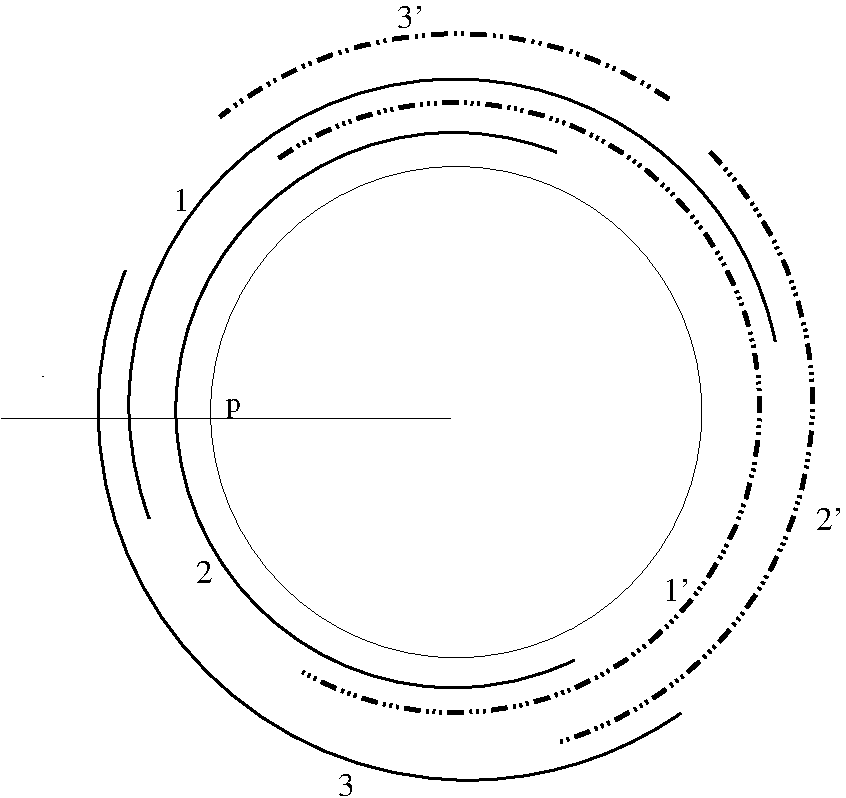
\includegraphics[scale=0.4]{gfx/ARCS_NUM}
%{\input{t1.pstex_t}}
\caption{Example for numbering of vertices of a CA graph}
\label{Fig1}
\end{center}
\end{figure}
Now, observe that in $G$, if a vertex $i \in A$ is adjacent to a vertex $j' \in B$, then at least one of the following is true: 
(a) the point $t(i)$ is contained in the arc $[s(j'), t(j')]$ or (b) the point $t(j')$ is contained in the arc $[s(i), t(i)]$. This implies that if $i \in A$ is adjacent to $j' \in B$, then  either (a) $j'$ is adjacent to all $k$ such that $1\le k \le i$  or (b) $i$ is adjacent to all $k'$ such that $1\le k' \le j'$. Thus the numbering scheme defined above, satisfies bi-consecutive adjacency property between $A$ and $B=V \setminus A$. Given the CA model $M(C$, $\mathcal{A})$, and a point $p$ on $C$, this numbering scheme can be computed in $O(n^2)$ time.
\end{proof}
\begin{claim}\label{claim2}
Let $G_0(V, E_0)$ be the supergraph of $G(V, E)$ constructed at the beginning of this section. Consider the numbering scheme $NS(M$, $p)$ of vertices $G$, as obtained by Lemma \ref{prop1}. The same numbering of vertices will satisfy the bi-consecutive adjacency property between $A$ and $V\setminus A$ in the graph $G_0$ as well.
\end{claim}
\begin{proof}
Recall our construction of the supergraph $G_0(V, E_0)$ of $G(V, E)$. For any pair of vertices $i \in A$ and $j' \in V \setminus A$, $(u$, $v') \in E$ if and only if $(u$, $v') \in E_0$. Since the numbering scheme $NS(M$, $p)$ of vertices of $G$ satisfies bi-consecutive adjacency property between $A$ and $V \setminus A$ by Lemma \ref{prop1}, and the edges across $A$ and $V \setminus A$ are the same in both $G$ and $G_0$, the same numbering of vertices will satisfy the bi-consecutive adjacency property between $A$ and $V\setminus A$ in $G_0$ as well. 
\end{proof}
Recall that $G_0$ is constructed to be a co-bipartite graph, where $A$ and $V \setminus A$ are cliques. The following lemma explains how bi-consecutive adjacency property between $A$ and $V \setminus A$ gives $G_0$ the additional structure of being a circular arc graph.
\begin{lemma} \label{lmprop2}
Let $G$ be a co-bipartite graph with a partitioning of vertex set into cliques $A$ and $B=V \setminus A$ with $|A| = n_1$ and $|B|=n_2$. Suppose there exist a numbering scheme of vertices of $G$ which satisfies the bi-consecutive adjacency property between $A$ and $B$. Then $G$ is a CA graph.
\end{lemma}
 \begin{proof}
The proof is by construction of a CA model $M(C$, $\mathcal{A})$ for $G$.\\
\textbf{Step 1:} Choose four distinct points $a$, $b$, $c$, $d$ in the clockwise order on $C$. Initially fix $s(i) = a$  for all $i \in A$ and $s(j') = c$  for all $j' \in B$. Choose $n_1$ distinct points $p_{n_1}$, $p_{n_1 - 1}$, $\cdots$, $p_1$ in the clockwise order on the arc $(a$, $b)$ and set $t(i)=p_i$ for all $ i \in A$. Choose $n_2$ distinct points $p_{n'_2}$, $p_{{n_2 - 1}'}$, $\cdots$, $p_{1'}$ in the clockwise order on the arc $(c$, $d)$ and set  $t(j')=p_{j'}$ for all $ j' \in B$. As of now, the family of arcs that we have constructed represents two disjoint cliques corresponding to $A$ and $B$.\\
\textbf{Step 2:} Now we will modify the start points of each arc as follows: Consider vertex $i \in A$. If $j' \in B$ is the highest numbered vertex in $B$ such that $i$ is adjacent to all $k'$ with $1' \le k' \le j'$, then set $s(i) = t(j')= p_{j'}$. Similarly, Consider vertex $j' \in B$. If $i \in A$ is the highest numbered vertex in $A$ such that $j'$ is adjacent to all $k$ with $1 \le k \le i$, then set  $s(j') = t(i)= p_i$. Notice that we are not making any adjacencies not present in $G$ between vertices of $A$ and $B$ in this step.

 Since $A$ and $B$ are cliques, what remains to prove is that if a vertex $i \in A$ is adjacent to a vertex $j' \in B$, their corresponding arcs overlap. Consider such an edge $(i$, $j')$. If $j'$ is adjacent to all $k$ such that $1\le k \le i$, we would have extended $s(j')$ to meet $t(i)$ in Step~2 above. If this does not occur, then by assumed bi-consecutive adjacency property, $i$ is adjacent to all $k'$ such that $1\le k' \le j'$. In this case, we would have extended $s(i)$ to meet $t(j')$ in Step~2. In both cases, the arcs corresponding to vertices $i$ and $j'$ overlap. We got a CA model of $G$ proving that $G$ is a CA graph.
\end{proof}
\begin{remark}\label{rmk2}
A different presentation of Lemma \ref{lmprop2} and an independent proof was obtained by Shrestha et al. \cite{Shrestha10}, 
while studying a class of graphs called $2$-directional orthogonal ray graph (2DORGS). Our proof presented above was obtained independently of 
their proof. Shrestha et al. \cite{Shrestha10} showed that a bipartite graph $G$ is a 2DORGS if and only if its complement $\overline{G}$ 
is a co-bipartite CA graph. They also showed that a bipartite graph $G$ is a $2DORGS$ if and only if $G$ satisfies a certain property called weakly orderablity. 
From the definition of weakly orderablity it follows that the notions of weakly orderablity of $G$ and the bi-consecutive adjacency property of $\overline{G}$ 
coincide and Lemma \ref{lmprop2} follows.
\end{remark}
By Claim \ref{claim2}, a numbering scheme of vertices of the co-bipartite graph $G_0$ is computable in $O(n^2)$ time such that it satisfies the 
bi-consecutive adjacency property between cliques $A$ and $V\setminus A$ in $G_0$. By Lemma \ref{lmprop2}, this implies that $G_0$ is a 
co-bipartite CA graph. Hence, using the algorithm of Section~\ref{sec:intro}, we can compute an optimal box representation $\mathcal{B}_0$ in polynomial time. By Lemma \ref{lem4version1}, $|\mathcal{B}_0| \le 2 \operatorname{box}(G)$. Since $G= G_0 \cap G_1$, by Claim \ref{claim1}, $\mathcal{B}= \mathcal{B}_0 \cup \{G_1\}$ is a valid box representation of $G$ of dimension $|\mathcal{B}_0|+1 \le 2 \operatorname{box}(G) +1$. We already saw that we can compute $G_1$ and its interval representation in linear time. Thus, $\mathcal{B}$ is a box representation of $G$ of dimension at most $2 \operatorname{box}(G)+1$ and it is computable in polynomial time. 

As in the proof of Theorem \ref{thm:mythm}, we can show that $\operatorname{box}(G_0)$ can be computed in $O(\xi n+n^2)$ time and an optimal box representation $\mathcal{B}_0$ of $G_0$ can be computed in $O(\xi n+k_0 n^2)$ time, where $n=|V(G_0)|=|V(G)|$, $k_0=\operatorname{box}(G_0) \le \operatorname{box}(G)=k$ and $\xi$ is a quantity which is at most the number of edges between $A$ and $V \setminus A$ in $G_0$. From our definition of $G_0$, in this case also we have $\xi \le m$. Therefore, the time required for computing $\operatorname{box}(G_0)$ and $\mathcal{B}_0$ are respectively within $O(mn+n^2)$ and $O(mn+kn^2)$. From this, we can see that $|\mathcal{B}|$ can be computed in $O(mn+n^2)$ time and $\mathcal{B}$ can be computed in $O(mn+kn^2)$ time, since the interval representation of $G_1$ was computed in linear time. Thus, we have the following theorem.
\begin{theorem}\label{approxCA}
 Let $G$ be a CA graph. A $\left(2+\frac{1}{k}\right)$-factor approximation for $\operatorname{box}(G)$ can be computed in $O(mn+n^2)$ time and a box representation of $G$ of dimension at most $2 \operatorname{box}(G)+1$ can be computed in $O(mn+kn^2)$ time, where $m=|E(G)|$, $n=|V(G)|$ and $k=\operatorname{box}(G)$.
\end{theorem}
\section[Complexity of the algorithm]{Complexity of computing the boxicity and optimal box representation of co-bipartite CA graphs} \label{complexity}
In Section~\ref{sec:intro}, we gave a polynomial time algorithm to compute an optimal box representation of a co-bipartite CA graph. 
In this section, we will analyze the time complexity of this algorithm and using some structural properties, show how this method 
can be made more efficient. First, let us do a preliminary analysis of our algorithm of Section~\ref{sec:intro}. 

Let $G(V$, $E)$ be a co-bipartite CA graph with $|E| = m$ and $|V|= n$. Let $H=\overline G$. Recall that by Theorem \ref{thm:mythm}, 
$\operatorname{box}(G)= \chi(H^*)$. Let $C_1$, $C_2$, $\cdots$, $C_k$ be the color classes in an optimal coloring of $H^*$. 
For $1\le i\le k$, let $C'_i$ be a maximal independent set containing $C_i$ and $E_i=\{e \in E(H)  \mid \Gamma_e \in C'_i\}$. 
By Theorem \ref{thm:mythm}, $\{G_i=\overline {H_i} \mid H_i=(V, E_i)$, $1 \le i \le k \}$ gives an optimal box representation of $G$. Our aim is to reduce the complexity of computing an optimal proper coloring of $H^*$, which is a crucial step in our algorithm. We also require an efficient method to extend the color classes of $H^*$ to maximal independent sets. 

By Theorem \ref{thm:mythm}, $H^*$ is a perfect graph. Let $t$ be the number edges of $H$ or equivalently, the number of vertices in $H^*$. Using the standard perfect graph coloring methods, $\chi(H^*)$ can be computed, as done in \cite{Abu10}. However, this method takes $O(t^3)$ time, which could be as bad as $O(n^6)$ in the worst case, where $n$ is the number of vertices of $G$. In \cite{Abu10}, for the restricted case when $H$ is an interval bigraph, they succeeded in reducing the complexity to $O(tn)$, using the zero partitioning property of the adjacency matrix of interval bigraphs. Unfortunately, since the zero partitioning property is the defining property of interval bigraphs, we cannot use the method used in \cite{Abu10} in our case, because the complements of CA co-bipartite graphs form a strict superclass of interval bigraphs \cite{Shrestha10}. Hence to bring down the complexity of the algorithm from $O(t^3)$, we have to go for a new method. 
The following tests algorithms.
\begin{algorithm}\small
     %\linesnumbered
     %\SetNoline
     %\dontprintsemicolon
%\singlespacing
     \LinesNumbered 
     %\SetAlgoNoLine
     \DontPrintSemicolon
 \caption{Computing colors of non-edges incident on vertex $x \in A$}
\label{alg1} 
     \KwIn{$x \in A$ }
    \KwOut{$Color(xy')$ for each $y' \in \widehat N_{_{B}}(x)$}
        \tcc{Type 0 work : Lines \ref{Ins} to \ref{Ine} - Initializations}
         \tcc{Let $P=\{a \in N_{_{A}}(\widehat N_{_{B}}(x)) \mid a < x\}$}
          {For $1\le a \le n_1$, let $A_P[a]=0$ initially. For each $a \in P$, set $A_P[a]=1$ and $color[a] = 1$\label{Ins}}\; 
    {Compute  $Q=\{b' \in N_{_{B}}(x) \mid b'< p'\}$, where $p' =\min{(\widehat N_{_{B}}(x))}$, which is the first element of $\widehat N_{_{B}}(x)$. For each $b' \in Q$, initialize  $ptr1[b']=\text{NULL}$ if $\widehat N_{_{A}}(b')=\emptyset$, and $ptr1[b']=$ start of $\widehat N_{_{A}}(b')$ otherwise \label{s2}}\;
         {Assign $R=\widehat N_{_{B}}(x)$ and for each $r' \in R$ initialize $Color(xr')=1$ and initialize $ptr2[r']=\text{NULL}$ if $N_{_{A}}(r')=\emptyset$ and $ptr2[r']=$ start of $N_{_{A}}(r')$ otherwise \label{Ine}}\;
       \For{cur $= 1$ to $n_1$}{                           
            \If {$A_{P}[\text{cur}]=1$}{
                \tcc{Type 1 work : Lines \ref{sf} to \ref{ef} - Computing $color[cur]= 1+ $ the maximum color given to a non-edge between $cur$ and $Q$}        
                 \For {each $q'$ in $Q$\label{sf}}{ 
                      \While {$ptr1[q']$ is not $\text{NULL}$ \label{wh1} and $\widehat N_{_{A}}(q')[ptr1[q']]< cur$}
                      { 
                        Increment the pointer $ptr1[q']$    \tcc*{$ptr1[q']$ becomes $\text{NULL}$ if it is incremented past the last element in $\widehat N_{_{A}}(q')$}
                      }                       
		      \uIf{$ptr1[q']$ is $\text{NULL}$ \label{l10}}
                       { delete $q'$ from $Q$ \label{l11}\;}
                      \ElseIf{$\widehat N_{_{A}}(q')[ptr1[q']] = cur$}{
			  $color[cur] = \max(color[cur],$ $Color(cur$ $q') + 1)$ \tcc*[assign]{non-edge $(cur$ $q')$ is already colored} 
                      }\label{l14}
                 }\label{ef}  
		\tcc{Type 2 work : Lines \ref{sf1} to \ref{ef1} - Identify non-edges at $x$ affected by non-edges between $cur$ and $Q$ and update their colors if necessary}  
                   \For {each $r'$ in $R$}{\label{sf1}
	                 \While {$ptr2[r']$ is not $\text{NULL}$ and $N_{_{A}}(r')[ptr2[r']]< cur $\label{wh2}} 
                          {Increment the pointer $ptr2[r']$  \tcc*{$ptr2[r']$ becomes $\text{NULL}$ if it is incremented past the last element in $N_{_{A}}(r')$}
                          }
		          \uIf{$ptr2[r']$ is $\text{NULL}$ \label{l20}}
                             { delete $r'$ from $R$ \label{l21} \;}
			  \ElseIf{$N_{_{A}}(r')[ptr2[r']] = cur$\label{l22}}{ 
                             \lIf{$Color(xr')< color[cur]$  \label{l23}}{
			       $Color(xr') = color[cur]$\;}
		           } \label{l24}
                        }\label{ef1}
                 }%\ENDIF
	     }%\ENDFOR   
           \end{algorithm}
           
The next question is to efficiently compute $MaxS_i$, for $1\le i\le k$. For this purpose, we introduce the following definition.
\begin{definition}\label{lnext}
For each $ab' \in E(H)$, let
\begin{displaymath}
Next(ab') = \left\{ \begin{array}{ll}
 \min\{Color(e):{e \in E(H), ab' \prec e }\},\\ {\mathrm{\hspace{3cm}if \ }\exists e \in E(H) \mathrm{\ such \ that \ }ab' \prec e}\\
 k+1,\mathrm{ \hspace{3.7cm} otherwise}
  \end{array} \right.
\end{displaymath}
\end{definition}         
\subsection{An $O(n^4)$ time algorithm for computing $\chi(H^*)$}\label{secondalgo}
Our method proceeds by computing a numbering of the vertices of $G$ such that bi-consecutive adjacency property is satisfied between the clique partitions of $G$. This numbering scheme is then used to prove that $H^*$ is a comparability graph and hence time required for computing an optimal proper coloring of $H^*$ can be brought down to $O(t^2)=O(n^4)$. Later, we will see that the same numbering scheme can be used to reduce the time complexity of our algorithm further. 

The following property holds for any co-bipartite CA graph.
 \begin{lemma} \label{CAclique}
 If $G(V$, $E)$ is a co-bipartite CA graph, then we can find a partition $A\cup B$ of $V$ where $A$ and $B$ induce cliques, having a numbering scheme of the vertices of $A$ and $B$ such that it satisfies bi-consecutive adjacency property between $A$ and $B$. Moreover, the numbering scheme can be computed in $O(n^2)$ time. 
\end{lemma}
\begin{proof}
  Let $G$ be a co-bipartite CA graph. Recall that a circular arc model of $G$ is constructible in linear time \cite{Ross1}. In any circular arc model  $M(C$, $\mathcal{A})$ of a co-bipartite CA graph $G$, there are two points $p_1$ and $p_2$ on the circle $C$ such that every arc passes through at least one of them \cite{Tucker2,Lin09}. It is easy to see that these points can be identified in $O(n^2)$ time. Let the clique corresponding to $p_1$ be denoted as $A$. Let $B=V \setminus A$, which is clearly a clique, since the arcs corresponding to all vertices in $B$ pass through $p_2$. Let $|A|=n_1$ and $|B|=n_2$. Then, by Lemma \ref{prop1}, we can compute a numbering scheme $NS(M$, $p_1)$ in $O(n^2)$ time, such that the vertices of $A$ are numbered $1$, $2$, $\cdots$, $n_1$ and vertices of $B$ are numbered $1'$, $2'$, $\cdots$, $n_2'$ and it satisfies bi-consecutive adjacency property between $A$ and $B$. 
\end{proof}
In order to show that $H^*$ is a comparability graph, we define a binary relation on $V(H^*)$. 
\begin{definition}\label{defRelation}
  Let $A \cup B$ be a partitioning of the vertex set $V(G)$ as described in Lemma \ref{CAclique}, where $A$ and $B$ are cliques in $G$ and $A=\{1$, $2$, $\cdots$, $n_1\}$ and $B=\{1'$, $2'$, $\cdots$, $n_2'\}$ is the associated numbering of vertices. We define a relation $\prec$ on $E(H)$ as: $ ab' \prec cd'$ if and only if $a$, $c \in A$, $b'$, $d' \in B$ with $a < c$ and $b'< d'$ and $\{a$, $b'$, $c$, $d'\}$ induces a $2K_2$ (i.e. a matching containing two edges) in $H$. Correspondingly, we also define a relation $\prec^*$ on $V(H^*)$ as: $\Gamma_{ab'} \prec^* \Gamma_{cd'}$ if and only if $ab' \prec cd'$.
\end{definition}
 From the definition of $H^*$ and the definition of $\prec^*$, it follows that if $\Gamma_{ab'} \prec^* \Gamma_{cd'}$, then $\Gamma_{ab'}$ and $\Gamma_{cd'}$ are adjacent vertices in $H^*$. We claim that the converse is also true. 
\begin{claim}\label{claimAdjRel}
If vertices $\Gamma_{ab'}$ and $\Gamma_{cd'}$ are adjacent in $H^*$, then they are comparable with respect to the relation $\prec^*$.
\end{claim}
\begin{proof}
 Let $\Gamma_{ab'}$ and $\Gamma_{cd'}$ be two adjacent vertices of $H^*$ corresponding to the edges $ab'$ and $cd'$ of $H$ where $a$, $c \in A$, $b'$, $d' \in B$. 
From the definition of $H^*$, it follows that $\{a$, $b'$, $c$, $d'\}$ induces a $2K_2$ in $H$. Equivalently, these vertices induce a 4-cycle in $G$ with edges 
$ac$, $cb'$, $b'd'$ and $d'a$. We have either $a < c$ or $c < a$. 

We claim that $a < c$ if and only if $b' < d'$. To see this, assume that $a < c$. Since $cb' \in E(G)$, by the Bi-Consecutive property of 
the numbering scheme (Lemma \ref{prop1}), if $d' < b'$, $cd' \in E(G)$ or $ab' \in E(G)$, a contradiction. Hence, $b' < d'$. From this, 
it follows that if $a < c$, then $ab' \prec cd'$ and therefore, $\Gamma_{ab'} \prec^* \Gamma_{cd'}$. Using similar arguments, we can show that if $c < a$, 
then $\Gamma_{cd'} \prec^* \Gamma_{ab'}$. 
\end{proof}
\begin{claim}\label{claim3}
The binary relation $\prec^*$ on $V(H^*)$ is antisymmetric and transitive. 
\end{claim}
\begin{proof}
It is clear from Definition \ref{defRelation} that the relations $\prec$ and $\prec^*$ are antisymmetric.

To show that $\prec^*$ is transitive, let $\Gamma_{ab'} \prec^* \Gamma_{cd'}$ and $\Gamma_{cd'} \prec^* \Gamma_{ef'}$.  
From the definition of $\prec^*$, the vertex set $\{a$, $b'$, $c$, $d'\}$ induces a $2K_2$ in $H$ with edges $ab'$ and $cd'$. 
Equivalently the vertex set $\{a$, $b'$, $c$, $d'\}$ induces 4-cycle in $G$ with edges $ac$, $cb'$, $b'd'$ and $d'a$. Similarly, 
the vertex set $\{c$, $d'$, $e$, $f'\}$ induces a 4-cycle in $G$  with edges $ce$, $ed'$, $d'f'$ and $f'c$. We also have  $a<c<e$ and $b'<d'<f'$, 
by the definition of the relation $\prec^*$. By the Bi-Consecutive property of the numbering scheme (Lemma \ref{prop1}), $cf' \in E(G)$ and $cd' \notin E(G)$ implies that 
$af' \in E(G)$. Similarly, $ed' \in E(G)$ and $cd' \notin E(G)$ implies that $eb' \in E(G)$. Edges $ae$ and $b'f'$ are parts of cliques $A$ and $B$. 
Hence, we have an induced 4-cycle in $G$ with edges $ae$, $eb'$, $b'f'$ and $f'a$. We can conclude that $ab' \prec ef'$ which implies $\Gamma_{ab'} \prec^* \Gamma_{ef'}$. 
Thus the relation $\prec^*$ is transitive.
\end{proof}
\section{Conclusion}
We showed that, for a co-bipartite CA graph $G$, an optimal box representation of $G$ can be obtained in polynomial time. 
Later, using some structural properties of co-bipartite CA graphs, we made this algorithm more efficient and showed that $\operatorname{box}(G)$ can be computed in $O(mn+n^2)$ time and an optimal box representation of $G$ can be obtained in $O(mn+kn^2)$ time, where $m=|E(G)|$, $n=|V(G)|$ and $k=\operatorname{box}(G)$. 
The algorithms developed for co-bipartite CA graphs are used as subroutines in all the remaining algorithms in this chapter. We gave an algorithm to compute a box representation of an arbitrary CA graph $G$, of dimension at most $2 \operatorname{box}(G)+1$. 
We also explained how to compute box representations of proper CA graphs, of dimension at most two more than the optimum. 
We also gave an algorithm to compute a cube representation of a CA graph $G$ of dimension at most $2 \operatorname{cub}(G)+\lceil \log{n} \rceil$. 
The time required for approximating the boxicity (resp. 
cubicity) is $O(mn+n^2)$ and the time required for computing 
the box (resp. cube) representation is $O(mn+kn^2)$, in all the above algorithms.  
